\sect{Compute Node Architecture}

\subsect{Tree Parameters}

In order to reap the full benefit of the tree data structure, an informed choice
of parameters must be made that takes consideration of the expected workload and
usage of scarce memory resources.

The tree's branching factor $m$ defines the maximum number of children that each
node can have. A level $k$ down the tree from the root will contain $m^k$ nodes.
Thus, a tree of height $h$ will contain
$\sum_{k=1}^h m^k = \frac{1-m^h}{1-m}$ nodes.

The ratio of leaf nodes to internal nodes is given by:
$$
	\frac{m^{h-1}}{\pfrac{1-m^{h-1}}{1-m}}
	= \frac{m^{h-1}(1-m)}{1-m^{h-1}}
	= \frac{m^{h-1}-m^{h}}{1-m^{h-1}}
	% = \frac{m^h-m^{h+1}}{m-m^h}
	% = \frac{m^h(1-m)}{m^h(m^{1-h} - 1)}
	= \frac{1-m}{m^{1-h} - 1}
$$

As $h$ increases, this rapidly converges to $m-1$.

\begin{figure}[H]
	\centering
	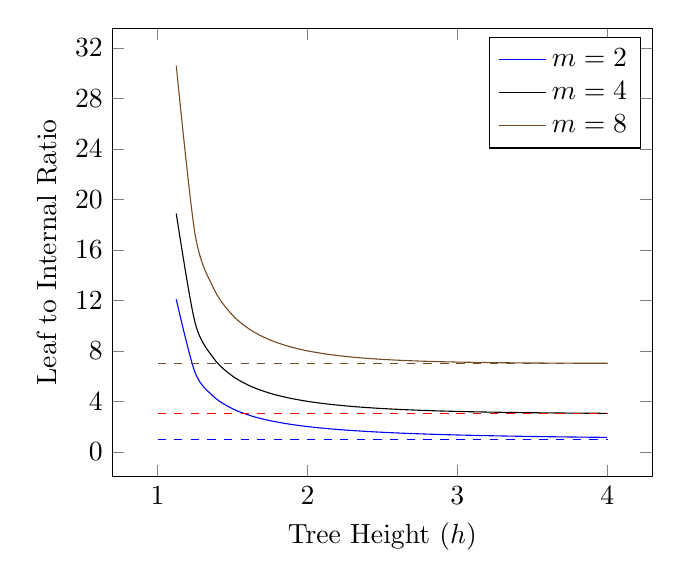
\begin{tikzpicture}
	\begin{axis}
		[
			xlabel={Tree Height ($h$)},
			ylabel={Leaf to Internal Ratio},
			xtick distance=1,
			ytick distance=4,
			domain=1:4,
			smooth
		]
		\pgfplotsinvokeforeach{2,4,8} {
			\addplot+[cycle list name=color list, mark=none]
				{(1-#1) / (#1^(1-x) - 1)};
			\addlegendentry{$m=#1$}
		}
		\pgfplotsset{cycle list shift=-3};
		\pgfplotsinvokeforeach{2,4,8} {
			\addplot+[cycle list name=color list, mark=none, dashed] {#1-1};
		}
	\end{axis}
\end{tikzpicture}

\end{figure}

As the height of a tree grows, the portion of overall memory that is used for
leaves decreases, converging to $1-\frac{1}{m}$. Higher branching factors spend
less memory on traversal data. Recall that internal nodes do not store data;
they store pointers to other nodes to accelerate lookups over a flat ordered
list. Such a flat list of $n$ elements is equivalent to a B-Link tree of $m=n$
and $h=1$.

\begin{figure}[H]
	\centering
	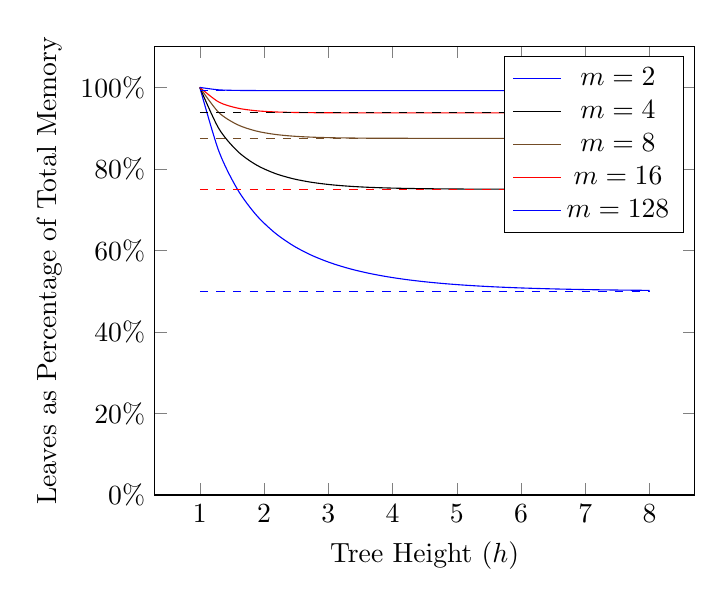
\begin{tikzpicture}
	\begin{axis}
		[
			xlabel={Tree Height ($h$)},
			ylabel={Leaves as Percentage of Total Memory},
			xtick distance=1,
			yticklabel={%
				\pgfmathparse{\tick*100}%
				\pgfmathprintnumber{\pgfmathresult}%
				\%%
			},
			domain=1:8,
			ymin=0,
			smooth
		]
		\pgfplotsinvokeforeach{2,4,8,16,128} {
			\addplot+[cycle list name=color list, mark=none]
				{#1^(x-1) / ((1-#1^x)/(1-#1))};
			\addlegendentry{$m=#1$}
		}
		\pgfplotsset{cycle list shift=-5}
		\pgfplotsinvokeforeach{2,4,8,16,128} {
			\addplot+[cycle list name=color list, mark=none, dashed]
				{1-(1/#1)};
		}
	\end{axis}
\end{tikzpicture}

\end{figure}

A tree containing $N$ nodes will have the height shown below.

\begin{align*}
	N &= \frac{1-m^h}{1-m} \\
	N (1-m) &= 1-m^h \\
	N (1-m) - 1 &= -m^h \\
	1 - N (1-m) &= m^h \\
	\log_m\left(1 - N (1-m)\right) &= h
\end{align*}

As $N$ grows, this relation can be approximtaed as $h \approx 1 + \log_m(N)$,
which is equivalent to  $m^{h-1} \approx N$. Because $m^{h-1}$ is the number of
leaf nodes, this expression approximates the total count of nodes as the number
of leaf nodes. As follows from previous derivations, this approximation is more
accurate for larger $m$ where there are more leaves per inner node.

\begin{figure}[H]
	\centering
	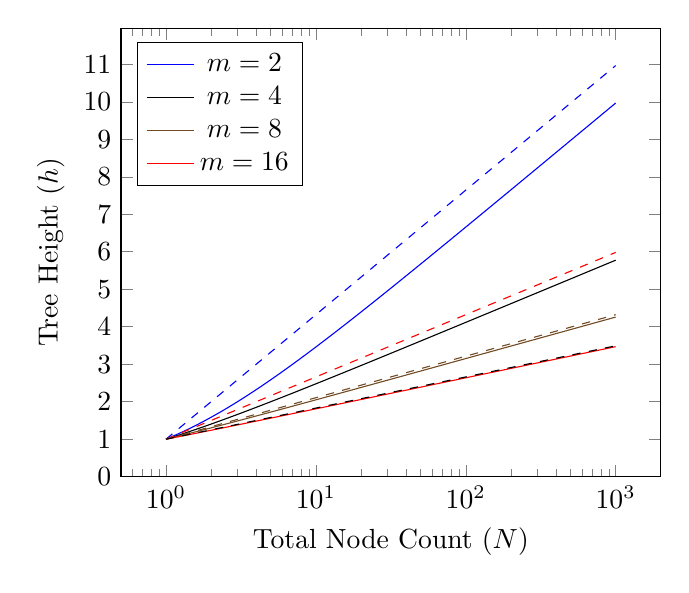
\begin{tikzpicture}
	\begin{axis}
		[
			xlabel={Total Node Count ($N$)},
			ylabel={Tree Height ($h$)},
			domain=1:1000,
			xmode=log,
			ytick distance=1,
			legend pos=north west,
			smooth
		]
		\pgfplotsinvokeforeach{2,4,8,16} {
			\addplot+[cycle list name=color list, mark=none]
				{ln(1 - x*(1-#1)) / ln(#1)};
			\addlegendentry{$m=#1$}
		}
		\pgfplotsset{cycle list shift=-4}
		\pgfplotsinvokeforeach{2,4,8,16} {
			\addplot+[cycle list name=color list, mark=none, dashed]
				{1+ln(x)/ln(#1)};
		}
	\end{axis}
\end{tikzpicture}

\end{figure}

\begin{figure}[H]
	\centering
	\begin{tikzpicture}
	\begin{axis}
		[
			xlabel={Total Node Count ($N$)},
			ylabel={Tree Height Approximation Error},
			domain=1:1000000,
			xmode=log,
			yticklabel={%
				\pgfmathparse{\tick*100}%
				\pgfmathprintnumber{\pgfmathresult}%
				\%%
			},
			smooth,
			cycle list name=rainbow4,
		]
		\pgfplotsinvokeforeach{2,4,8,16} {
			\addplot+[cycle list name=color list, mark=none]
				{
					(
						(
							1+ln(x)/ln(#1)
						) - (
							ln(1 - x*(1-#1)) / ln(#1)
						)
					) / (
						ln(1 - x*(1-#1)) / ln(#1)
					)
				};
			\addlegendentry{$m=#1$}
		}
	\end{axis}
\end{tikzpicture}

\end{figure}


\subsect{Memory Layout}

Even without the considerations of caching that would arise on CPU-based
systems, memory access patterns can stil have significant performance impacts.
The XCU280 FPGA integrates $\SI{8}{\giga\byte}$ of on-chip High-Bandwidth Memory
(HBM) with a theoretical maximum bandwidth of $\SI{460}{\giga\byte\per\second}$
\autocite{u280}, but this is contingent on spreading out the accesses across all
available channels \autocite{holzinger-ipdpsw-2021}.

Though using HLS prevents some of the lower-level access optimizations proposed
by \citeauthor{holzinger-ipdpsw-2021}, it is still possible to reap some
benefits by controlling memory access patterns. Because the manner that the
abstract tree is accessed is dictated by \citeauthor{b-link}'s original
algorithm, the best way to optimize memory accesses is to consider how best to
lay out the tree in memory.


\begin{figure}[H]
	\centering
	\begin{tikzpicture}[
		tree/.style={draw,circle,inner sep=0.25mm,minimum size=14pt}
	]
	\node[tree] at (0, 0) (00) {$0,0$};
	\foreach \r [
		evaluate = \r as \w using int(3^\r),
		evaluate = \r as \wl using int(3^\r-1)
	] in {1,...,2} {
		% Columns
		\foreach \c [
			evaluate = \c as \i using int((\w-1)/2 + \c),
			evaluate = \c as \pr using int(\r-1),
			evaluate = \c as \pc using int(\c/3),
		] in {0,...,\wl} {
			\node[tree] (\r\c)
				at ({0.7*\c}, -\r) {$\r,\c$};
			\draw[-] (\pr\pc.south)
				-- ++(0, {-((3-\pc) + (\pr-1))/9}) -| (\r\c);
		}
	}
	\node[anchor=east] (legend) at (00 -| 28) {Node text is $r,c$};
	\node[anchor=east, below=0.1 of legend] {$m=3, h=3$};
\end{tikzpicture}

\end{figure}

Two memory layout schemes have been implemented. The first maps the tree to a
simple rectangular matrix. Each row of the matrix corresponds to nodes at the
same same level of the tree. Node that these are not all inhrently siblings of
one another, as leaf nodes with different parents are still at the leaf-node
level of the tree. This strategy maintains locality for tree levels and allows
for easy determination of what level a node resides in, but wastes more memory
the closer a level is to the root.

This strategy also imposes a stricter height limit on the tree than may be
possible with a given amount of memory. Though B-tres are considered
``self-balancing'' in the academic sense, there is no guarantee of a constant
height for all sub-trees. The easiest demonstration of this is to observe the
insertion of a sequence of monotonically increasing keys.

\begin{figure}[H]
	\centering
	\begin{subfigure}{5em}
	\centering
	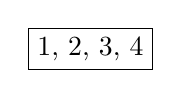
\begin{tikzpicture}
		\node[draw] (root) {1, 2, 3, 4};
	\end{tikzpicture}
	\caption*{One Node}
\end{subfigure}
\begin{subfigure}{7em}
	\centering
	\begin{tikzpicture}[node distance=0.25]
		\node[draw] (leaf1) {1, 2};
		\node[draw] (leaf2) [right=of leaf1] {3, 4, 5};
		\coordinate (center) at ($ (leaf1) !.5! (leaf2) $);
		\node[draw] (root) [above=0.5 of center] {2, 5};
		\draw (root) -- (leaf1);
		\draw (root) -- (leaf2);
	\end{tikzpicture}
	\caption*{After First Split}
\end{subfigure}
\begin{subfigure}{14em}
	\centering
	\begin{tikzpicture}[node distance=0.25]
		\node[draw] (leaf1) {1, 2};
		\node[draw] (leaf2) [right=of leaf1] {3, 4};
		\node[draw] (leaf3) [right=of leaf2] {5, 6};
		\node[draw] (leaf4) [right=of leaf3] {7, 8, 9, 10};
		\coordinate (center) at ($ (leaf2) !.5! (leaf3) $);
		\node[draw] (root) [above=0.5 of center] {2, 4, 6, 10};
		\draw (root) -- (leaf1);
		\draw (root) -- (leaf2);
		\draw (root) -- (leaf3);
		\draw (root) -- (leaf4);
	\end{tikzpicture}
	\caption*{Before Second Split}
\end{subfigure}
\begin{subfigure}{16em}
	\centering
	\begin{tikzpicture}[node distance=0.25]
		\node[draw] (leaf1) {1, 2};
		\node[draw] (leaf2) [right=of leaf1] {3, 4};
		\node[draw] (leaf3) [right=of leaf2] {5, 6};
		\node[draw] (leaf4) [right=of leaf3] {7, 8};
		\node[draw] (leaf5) [right=of leaf4] {9, 10, 11};
		\coordinate (center1) at ($ (leaf4) !.5! (leaf5) $);
		\coordinate (center2) at ($ (leaf2) !.5! (leaf3) $);
		\node[draw] (inner1) [above=0.5 of center1] {8, 11};
		\node[draw] (root) [above=1 of center2] {2, 4, 6, 11};
		\draw (root) -- (leaf1);
		\draw (root) -- (leaf2);
		\draw (root) -- (leaf3);
		\draw (root) -- (inner1);
		\draw (inner1) -- (leaf4);
		\draw (inner1) -- (leaf5);
	\end{tikzpicture}
	\caption*{After Second Split}
\end{subfigure}
\begin{subfigure}{9em}
	\centering
	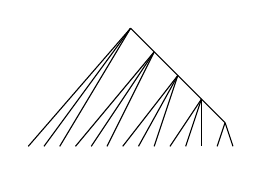
\begin{tikzpicture}[xscale=-0.2, yscale=0.3]
		\draw (1.5, 1) -- (1, 0);
		\draw (1.5, 1) -- (2, 0);
		\foreach \i in {2,...,5} {
			\draw ({\i*1.5}, \i) -- ({(\i-1)*1.5}, \i-1);
			\draw ({\i*1.5}, \i) -- ({3*(\i-1)}, 0);
			\draw ({\i*1.5}, \i) -- ({3*(\i-1)+1}, 0);
			\draw ({\i*1.5}, \i) -- ({3*(\i-1)+2}, 0);
		}
	\end{tikzpicture}
	\caption*{Overall Pattern}
\end{subfigure}

	\caption{Inner Node Structure for Sequential Insertions on an $m=4$ Tree}
\end{figure}
